\begin{frame}{Multiple Shaded Regions}
\begin{center}
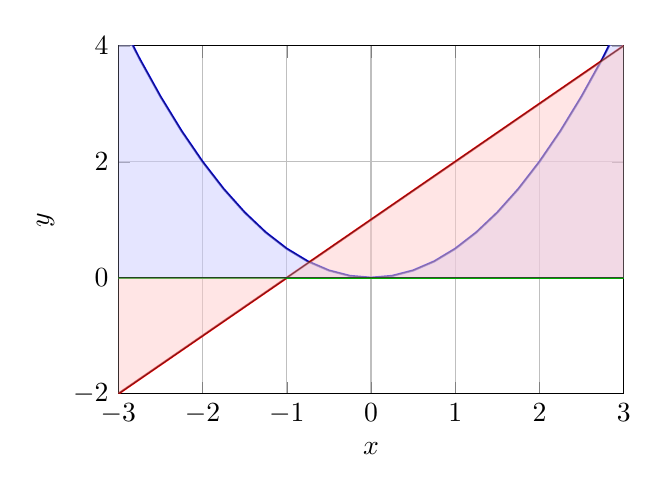
\begin{tikzpicture}
\begin{axis}[
    xlabel={$x$},
    ylabel={$y$},
    grid=both,
    xmin=-3, xmax=3,
    ymin=-2, ymax=4,
    width=8cm,
    height=6cm
]
\addplot[thick, blue, domain=-3:3] {x^2/2};
\addplot[thick, red, domain=-3:3] {x + 1};
\addplot[thick, green, domain=-3:3] {0};
\addplot[fill=blue!20, opacity=0.5, domain=-3:3] {x^2/2} \closedcycle;
\addplot[fill=red!20, opacity=0.5, domain=-3:3] {x + 1} \closedcycle;
\end{axis}
\end{tikzpicture}
\end{center}

\footnotesize
Multiple shaded regions with different colors
\end{frame}